\section{Computer Experiments}
\label{sec:experiments}

This section evaluates \abr{qa} systems on the \challenge{} questions. We
test three models: the \abr{ir} and \abr{rnn} models shown in the interface, as well as a Deep Averaging Network~\cite[\abr{dan}]{iyyer2015deep} to evaluate the transferability of the adversarial questions. We break our study into two rounds. The first round consists of \challenge{} questions written against
the \abr{ir} system (Section~\ref{subsec:one}); the second round questions target
both the \abr{ir} and \abr{rnn} (Section~\ref{subsec:two}).

Finally, we also hold live competitions that pit the state-of-the-art Studio Ousia model~\cite{yamada2018studio} against human teams (Section~\ref{subsec:live}).

% Depends on round 1 data so this produces only the labels for the plot since the data is round 2 data
% This is not auto fig, keeping command below for future reference
% /figures.py guesser --use-test --only-tacl --no-humans --title "Round 1 Attacks and Models" --rounds 1 output/tacl
\begin{figure*}[t!]
\centering  
\includegraphics[width=2\columnwidth]{round_1_csv}
\caption{The first round of adversarial writing attacks the \abr{ir} model. Like regular test
questions, \challenge{} questions begin with difficult clues that trick the model. However,
the adversarial questions are significantly harder during the crucial middle
third of the question.}
\label{fig:round_one}

% ./figures.py guesser --use-test --only-tacl --no-humans --title "Round 2 Attacks and Models" --rounds 2 output/tacl
%\begin{figure*}[t!]
\centering
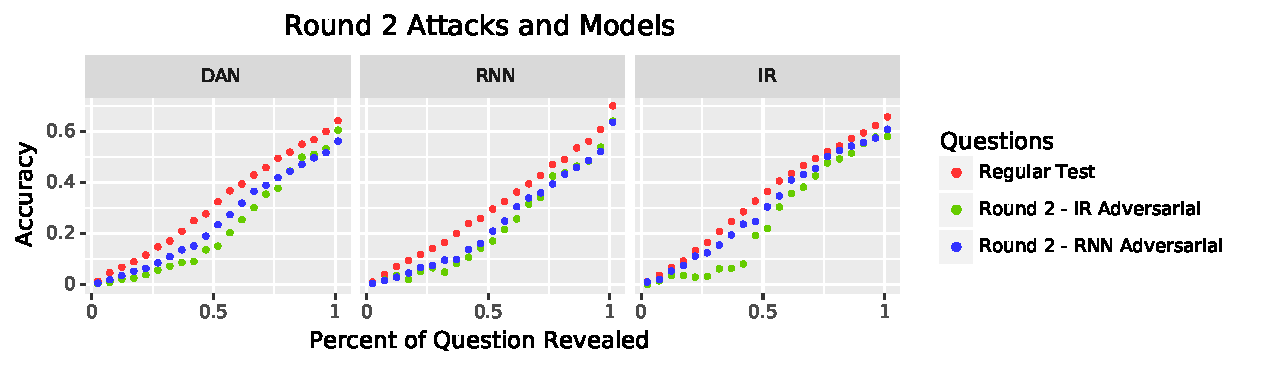
\includegraphics[width=2\columnwidth]{round_two}
\caption{The second round of adversarial writing attacks the \abr{ir} and \abr{rnn} models. The questions targeted against the \abr{ir} system degrade the performance of all models. However, the reverse does not hold: the \abr{ir} model is robust to the questions written to fool the \abr{rnn}.}
\label{fig:round_two}
\end{figure*}

\subsection{First Round Attacks: IR Adversarial
Questions Transfer To All Models}\label{subsec:one}

The first round of \challenge{} questions target the \abr{ir} model
and are significantly harder for the \abr{ir},
\abr{rnn}, and \abr{dan} models (Figure~\ref{fig:round_one}). For example,
the \abr{dan}'s accuracy drops from 54.1\% to 32.4\% on the full question
 (60\% of original performance).

For both \challenge{} and original test questions, the early
clues are difficult to answer (accuracy about
10\% through 25\% of the question). However, during the middle third 
of the questions, where buzzes in \qb{} most
frequently occur, the accuracy on original test questions rises
significantly quicker than the \challenge{} ones. For both questions,
the accuracy rises towards the end as the clues get simpler and become
``give-aways''.

 \subsection{Second Round Attacks: RNN Adversarial Questions are Brittle}\label{subsec:two}

In the second round, the authors also attack an \abr{rnn} model.
All models tested in the second round are trained on a larger dataset (Section~\ref{subsec:models}).

A similar trend holds for \abr{ir} adversarial question
in the second round (Figure~\ref{fig:round_two}): a question that tricks the \abr{ir} system also fools
the two neural models (i.e., the adversarial examples transfer). For example, the \abr{dan} model
was never targeted adversarially but had substantial
accuracy decreases in both rounds.

However, this does not hold for questions written adversarially
against the \abr{rnn} model. On these questions, the neural models
struggle but the 
\abr{ir} model is largely
unaffected (Figure~\ref{fig:round_two}, right).

\subsection{Humans vs. Computer, Live!}
\label{subsec:live}

% ./figures.py guesser --use-test --only-tacl --no-models output/tacl
\begin{figure*}
\centering
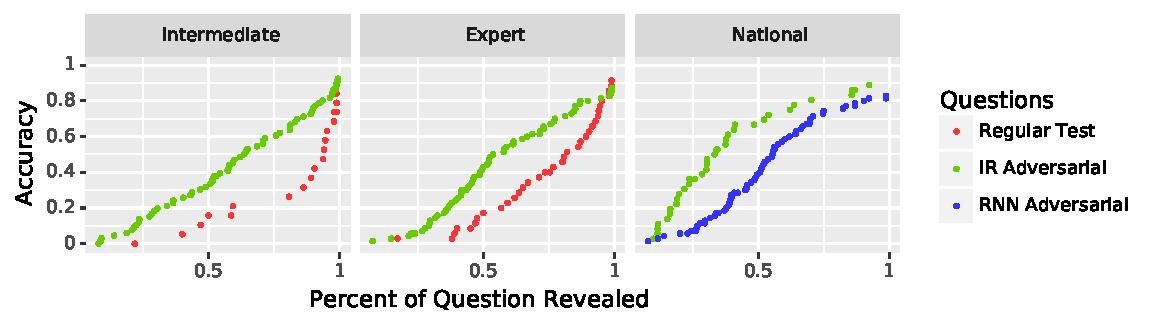
\includegraphics[width=2\columnwidth]{human_breakdown}
\caption{Humans find \challenge{} question about as difficult as
  normal questions regardless of whether they are rusty weekend
  warriors (\textit{Intermediate}), active players (\textit{Expert}), or
  some of the best trivia players in the world (\textit{National}).}
\label{fig:human_breakdown}
\end{figure*}

\begin{figure}[t!]
\centering
\includegraphics[width=\columnwidth]{ikuya_cdf}
\caption{The accuracy of the state-of-the-art Studio Ousia model degrades on the \challenge{} questions despite never being directly targeted. This verifies that our findings generalize beyond the \abr{rnn} and \abr{ir} models.}
\label{fig:ikuya_vs_human}
\end{figure}

In the offline setting (i.e., no pressure to ``buzz'' before an opponent) models
demonstrably struggle on the adversarial questions. But, what happens in
standard \qb{}: live, head-to-head 
games? 

We run two live humans vs. computer matches. The first match uses \abr{ir}
adversarial questions in a forty question, tossup-only \qb{} format. 
We pit a human team of national-level \qb{} players against the
Studio Ousia model~\cite{yamada2018studio},
the current state-of-the-art \qb{} system. The model combines neural,
\abr{ir}, and knowledge graph components (details in Appendix~\ref{sec:ousia}), and won the 2017 \abr{nips} shared task, defeating
a team of expert humans 475--200 on regular \qb{} test questions.
Although the
team at our live event was comparable to the \abr{nips}
2017 team, the tables were turned: the human team won handedly 300--30.

Our second live event is significantly larger:
seven human teams play against models on over 400 questions written adversarially against the \abr{rnn} model. The human teams range in ability from high school \qb{} players to national-level teams. The
models are based on either \abr{ir} or neural methods. Despite a few close games between the weaker human teams and the models, humanity prevailed in every match.\footnote{Videos available at \url{http://trickme.qanta.org}.}

Figures~\ref{fig:human_breakdown}--\ref{fig:ikuya_vs_human} summarize
the live match results for the humans and Ousia model, respectively. Humans
and models have considerably different trends in answer accuracy.
Human accuracy on both regular and adversarial questions rises
quickly in the \emph{last half}
of the question (curves in Figure~\ref{fig:human_breakdown}).
In essence, the ``give-away'' clues at the end of questions are easy for humans to answer.

On the other hand, models on regular test questions
do well in the \emph{first half}, i.e.,
the ``difficult'' clues for humans are easier for models (\emph{Regular Test} curve in Figure~\ref{fig:ikuya_vs_human}).
However, models, like humans, struggle to 
answer the adversarial questions in the first half of the question.
